\documentclass{article}
\usepackage{appendix}
\usepackage{amsthm,amsmath,amssymb,graphicx,amsfonts,epsfig,array,cite,wrapfig,epstopdf,verbatim,bm,epstopdf,subcaption}
\usepackage[hyphens]{url}
\usepackage{hyperref}
%\hypersetup{breaklinks=true}
\usepackage{algorithm,algorithmic} %,algorithmicx,algpseudocode}
\usepackage{multirow}
%\usepackage[center,footnotesize]{caption}
%\usepackage[textsize=small]{todonotes}
%\interdisplaylinepenalty=2500
%\usepackage{fullpage}

\usepackage{icml2017,natbib,fancyhdr,times}

\newtheorem{theorem}{Theorem}[section]
\newtheorem{lemma}{Lemma}[section]
\newtheorem{proposition}{Proposition}[section]
\newtheorem{corollary}{Corollary}[section]
\newtheorem{definition}{Definition}[section]
\newtheorem{remark}{Remark}[section]

\graphicspath{{figures/}}

%\newcommand{\Remark}[1]{\todo[inline,backgroundcolor=blue!20!white]{Remark: #1}}

\DeclareMathOperator{\Tr}{Tr}
\DeclareMathOperator{\Prox}{Prox}
\DeclareMathOperator{\diag}{diag}
\DeclareMathOperator{\Vol}{Vol}
\DeclareMathOperator{\Star}{Star}
\DeclareMathOperator{\argmin}{arg\,min}
\DeclareMathOperator{\argmax}{arg\,max}

\def \dx{\, \mathrm{d}}

%\algnewcommand\algorithmicinput{\textbf{Input:}}
%\algnewcommand\Input{\item[\algorithmicinput]}
%\algnewcommand\algorithmicoutput{\textbf{Output:}}
%\algnewcommand\Output{\item[\algorithmicoutput]}

%\title{Nearly-Linear Time Optimization for Connected Subgraph Detection}
%\author{}

\icmltitlerunning{Optimization for Connected Subgraph Detection}

\begin{document}

\twocolumn[
\icmltitle{Nearly-Linear Time Optimization \\ for Connected Subgraph Detection}

\icmlsetsymbol{equal}{*}

\begin{icmlauthorlist}
\icmlauthor{Aeiau Zzzz}{equal,to}
\icmlauthor{Bauiu C.~Yyyy}{equal,to,goo}
\icmlauthor{Cieua Vvvvv}{goo}
\icmlauthor{Iaesut Saoeu}{ed}
\icmlauthor{Fiuea Rrrr}{to}
\icmlauthor{Tateu H.~Yasehe}{ed,to,goo} 
\icmlauthor{Aaoeu Iasoh}{goo}
\icmlauthor{Buiui Eueu}{ed}
\icmlauthor{Aeuia Zzzz}{ed}
\icmlauthor{Bieea C.~Yyyy}{to,goo}
\icmlauthor{Teoau Xxxx}{ed}
\icmlauthor{Eee Pppp}{ed}
\end{icmlauthorlist}

\icmlaffiliation{to}{University of Torontoland, Torontoland, Canada}
\icmlaffiliation{goo}{Googol ShallowMind, New London, Michigan, USA}
\icmlaffiliation{ed}{University of Edenborrow, Edenborrow, United Kingdom}

\icmlcorrespondingauthor{Cieua Vvvvv}{c.vvvvv@googol.com}
\icmlcorrespondingauthor{Eee Pppp}{ep@eden.co.uk}

\icmlkeywords{boring formatting information, machine learning, ICML}

\vskip 0.3in
]

\printAffiliationsAndNotice{}

%\maketitle

\begin{abstract}
  We propose a novel, computationally efficient optimization framework for subgraph detection in graph-structured data, where we aim to discover anomalous patterns present in a connected subgraph of a given graph. This problem arises in many applications such as detection of network intrusions, community detection, detection of anomalous events in surveillance videos or disease outbreaks. %We specifically consider two different anomaly models: elevated mean detection and correlation detection. 
Since optimization over connected subgraphs is a combinatorial and computationally difficult problem, we propose a convex relaxation that offers a principled approach to incorporating connectivity and conductance constraints on candidate subgraphs. We develop a novel nearly-linear time algorithm to solve the relaxed problem, establish convergence and consistency guarantees and demonstrate its feasibility and performance with experiments on real networks.
\end{abstract}

\section{Introduction}

We consider the problem of connected subgraph detection, motivated by statistical anomaly detection on networks where the aim is to determine whether there exists a set of connected nodes that exhibit anomalous signal values. %with associated signals over its nodes or edges. 
%In the context of this thesis, this chapter replaces sparsity with connectedness as the signal ``structure'' in the problem of discovering low-dimensional structure in high-dimensional signals. 
One example of the anomaly detection problem on networks is disease outbreak detection \cite{disease}, where the nodes are associated with counties and geographical neighborhood characterizes connectivity, and signal values on nodes depict the number of patients related to a disease. In the existence of a disease outbreak that spreads geographically, higher signal values would be present on certain counties that are neighbors of each other, therefore constituting a subgraph structure. Similar problems in different research areas also exist, such as detection of intrusions in communication or sensor networks, community detection or video surveillance.  % add references for these

%\begin{figure}[t]
%  \centering
%  \includegraphics[width=0.4\textwidth]{disease.png}
%  \caption{Illustration of a disease outbreak and its graph representation. Each node corresponds to a county on the map and are connected to neighboring counties. The affected counties constitute a connected subgraph in the graph representation. The upper part of the figure is modified from \cite{disease} and the lower part is taken from \cite{aistats14}.}
%  \label{fig:disease}
%\end{figure}

The detection or estimation of arbitrary connected subgraphs over graph-structured signals is an example of a structured signal recovery problem and generalizes many useful types of structures such as intervals or paths \cite{addario,maze}. While the existence of structure in terms of connectivity leads to better statistical complexity in detecting or recovering the anomalous sets compared to arbitrary subsets, efficient characterization of sets obeying the connectivity constraint is important for obtaining practical algorithms for detection and estimation. In this paper we aim to characterize the space of arbitrary connected subsets of nodes in a graph in a principled manner through spectral graph theory and propose efficient optimization algorithms that exploit this characterization.


%In Section \ref{sec:subgraph} we formalize the subgraph detection problem and propose our convex relaxation into a SDP formulation, utilizing the LMI of \cite{aistats14} for connectivity. We empirically show that the relaxation we propose results in feasible solutions to the original problem after rounding. We then introduce mirror descent as a first-order optimization method in Section \ref{sec:mirror} and discuss it in the context of our formulation. Lastly in Section \ref{sec:future} we discuss future directions and plans, including a theoretical analysis of the relaxation and rounding, more efficient optimization by exploiting the graph structure and applications to specific anomaly detection problems.

\subsection{Related work and contributions}

% introduce prior work, compare to aistats and nips papers, extend below

Subgraph detection is a difficult problem since connected subgraphs represent a combinatorial structure and systematic approaches to characterizing the space of connected subgraphs of a given graph are relatively recent. 
%
% * <lorecchia@gmail.com> 2016-10-09T01:23:05.452Z:
%
% Can we be more specific here? What is known about the hardness of correlation detection? Later we use ref 5. However, Reference 5 does not seem to conclusively establish the hardness.
%
% ^.
Traditional approaches to this problem usually consider parametric methods, which originate from the scan statistics literature \cite{scan} and consider scanning for specific shapes such as rectangles, circles or neighborhood balls on graphs \cite{disease,kulldorf,priebe}. More recently nonparametric approaches have been considered for subgraphs with arbitrary shapes on general graphs. The simulated annealing approach of \cite{duczmal} is an example of nonparametric methods that can detect complex shapes, however it is a heuristic method without statistical or computational guarantees. There is also a line of work focused on statistical analysis with nonparametric shapes \cite{addario,maze,arias}, however they consider computationally intractable algorithms. 

More recently, \cite{aistats14,nips14} proposed a semidefinite programming (SDP) formulation of the problem, along with a novel linear matrix inequality (LMI) constraint that provably characterizes the connectivity of subsets of nodes exactly in the integer problem. This approach is the most similar to ours where we also consider an SDP relaxation with LMI constraints, however we take a different approach to formulating the problem and its relaxation, with the goal to obtain a convex optimization program that is amenable to more efficient iterative methods. Another notable work in this area is the spectral scan statistic approach proposed by \cite{sharpnack}, which presents a computationally tractable algorithm with consistency guarantees. However it is important to note that this method aims to obtain graph partitions with small conductance and balanced sizes, in contrast to our formulation that guarantees connected subgraphs. In recent work, \cite{wu} consider nonparametric statistics for signals in addition to nonparametric shapes, obtaining a computationally tractable algorithm by heuristically approximating the underlying graph with trees.

The contribution of this paper is twofold: First, we develop a convex relaxation of the subgraph detection problem that results in an semidefinite optimization formulation, with provable guarantees on the connectivity of the resulting solutions related to the internal conductance of the subgraph. Second, we propose an efficient iterative framework for optimizing the SDP that scales well with large problem sizes, and show computational guarantees. One of the major differences of our formulation to those of \cite{aistats14,nips14} is that prior work enforce a number of constraints that scale with the problem size, whereas ours only considers a constant number of constraints. Also, while aforementioned work utilized generalized convex optimization solvers, our formulation allows us to propose specialized and efficient iterative algorithms.  % CEM: remove last sentence(s)?

%To perform the optimization, we consider a first-order method in mirror descent for the convex formulation and later we propose to investigate possible connections to random walks on the graph, previously investigated for the balanced separator problem \cite{lorenzo}.


\section{Connected Subgraph Detection}

In this section we define the notation and introduce the two statistical models that we consider for the connected subgraph detection problem. Let $G = (V,E)$ denote an undirected unweighted connected graph with $n$ nodes that is provided as input to the problem. For $i \in V$, we write $d_i$ for the degree of vertex $i$ in $G$ and let $d$ be an upper bound on all $d_i$. For a subset $S \subseteq V$, the notation $\Vol(S)$ indicates the volume measure of $S$, i.e., $
\Vol(S) = \sum_{i \in S} d_i$.
We also denote by $G_S = (S, E_S)$ the subgraph induced by the subset $S$. For an input root vertex $r \in V$, we write $\Lambda_r = \{S \subseteq V : r \in S, \, G_S~\mathrm{is~connected~in}~G \}$. Indicator vectors with notation $1_S$ are defined as $n \times 1$ vectors with $i$-th index 1 if $i \in S$ and zero otherwise.

%the collection of all subsets of nodes that induce a connected subgraph over $G$. 

We consider observations $x_v \in \mathbb{R}^p$ associated with each node $v \in V$ in the graph $G$. We are concerned with optimization problems of the form
\begin{equation}
  \max_{S \in \Lambda_r} c(S),
  \label{eq:subg_opt}
\end{equation}
for a cost function $c(\cdot)$ which depends on $x_S = \{x_v\}_{v \in S}$. We remark that this is a difficult problem due to the combinatorial nature of the constraint, in fact variants of the prize-collecting Steiner tree problem which is known to be NP-hard \cite{pcst} can be reduced to the above formulation.
Below we provide two examples of the setup that we consider, namely elevated mean detection and correlation detection.

\paragraph{Elevated mean detection:}
In this problem, the aim is to detect the existence of a subgraph $S \in \Lambda_r$ comprising of nodes with an elevated mean compared to the other nodes. A simple example is the Gaussian elevated mean model, where $x_v = \mu 1\{v \in S\} + z_v$ for $\mu > 0$ and $z_v \sim \mathcal{N}(0, \sigma^2)$. Another example we consider is the Poisson variant, where $x_v \sim \mathrm{Poisson}((1 + \mu 1\{v \in S\}) \, \lambda)$.

We consider the optimization \eqref{eq:subg_opt} with the scan statistic
\begin{equation}
  c_1(S) = \frac{1}{\sqrt{|S|}} \sum_{i \in S} x_i,
  \label{eq:elevated}
\end{equation}
which can be shown to correspond to the generalized likelihood ratio test (GLRT) for the Gaussian detection problem, while also encouraging sparse solutions for estimation of $S$.

\paragraph{Correlation detection:}
Another example is the problem of detecting and estimating a subgraph with correlated signal values. The canonical statistical model that has been investigated for this problem is where the signals are jointly Gaussian random variables $X_1, \ldots, X_n$, where $\mathrm{cov}(X_i, X_j) = 1$ if $i = j$, $\rho$ if $i,j \in S$ and zero otherwise \cite{arias}. Note that while related work consider arbitrary $k$-sets or special shapes such as intervals for $S$, we allow arbitrary connected subgraphs containing the root $r$.

One simple test for detecting or estimating a correlated subgraph induced by set $S$ is \eqref{eq:subg_opt} with the scan statistic
\begin{equation}
  c_2(S) = \frac{1}{|S|} \sum_{i,j \in S} \hat{\Sigma}_{ij},
  \label{eq:correlation}
\end{equation}
where $\hat{\Sigma}$ is the estimated covariance matrix which can either be defined by a single observation $x x^\top$ when $p = 1$ or multiple observations for $p > 1$.

%LORENZO: need to introduce cut notation E(S,V \S)
%CEM: added notation below equation
\paragraph{Characterizing subgraph connectivity:}
Rather than focusing on exactly characterizing the connectedness of an induced subgraph $G_S$, we aim to enforce it by lower bounding the {\it conductance} of cuts within $G_S$.
For a weighted graph $G=(V,E,w)$, the conductance of a cut $S$ is defined as 
\[ \phi_G(S) = \frac{w(S,V \setminus S)}{\textrm{Vol(S)}}, \]
where $w(S, V \setminus S)$ is the total weight of edges connecting nodes in $S$ to nodes in $V \setminus S$. The graph conductance is the lowest conductance among cuts containing at most half of the volume of the graph, i.e., $\phi_G = \min_{S \subset V: \textrm{Vol}(S) \leq \textrm{Vol}(V)/2} \phi_G(S)$.
%
Conductance is a natural graph-partitioning objective because of its intimate connection with the behavior of random walks. It is also widely used in practice in the design of clustering and segmentation algorithms.
% add citations
We can use conductance to ensure subgraph connectivity by imposing the following constraints\footnote{Note that for technical reasons, the conductance $\phi_{G_S}$ on the induced graph $G_S$ still employs the definition of volume given by the larger graph $G$.} on the integral solution $S$:
% LORENZO: box this equation for emphasis?
\begin{equation}\label{eq:int}
  \phi_{G_S}(T) = \frac{w(T, S \setminus T)}{\textrm{Vol}(T)} \geq \gamma > 0, \quad \forall T \subseteq S \setminus \{r\}.
\end{equation}
For $\gamma$ sufficiently small, i.e., $\gamma < 1/\textrm{Vol}(V)$, this requirement is equivalent to the connectivity condition on $G_S$. 
It is useful to notice at this stage that the condition in constraint~\eqref{eq:int} is stronger than a lower bound on the conductance of the induced subgraph $G_S$. Indeed, for an unweighted graph the constraint~\eqref{eq:int} implies
\[ \phi_{G_S} = \min_{U \subseteq S: \Vol(U)  \leq \frac{\Vol(S)}{2}} \frac{|E(U, S \setminus U)|}{\Vol(U)} \geq \gamma, \]
where $E(U, S \setminus U)$ is the set of edges between sets of nodes $U$ and $S \setminus U$.
However, our constraint is stronger than requiring the induced conductance of $G_S$ to be $\gamma$, as the bound also holds for subsets $T \subset S$ comprising more than half the volume of $G_S$. 

\paragraph{Comparison with other measures of connectivity}
To form a better understanding of how conductance arises in this context, consider a (dual) flow formulation of connectedness: $S \in \Lambda_r$ if, for any $i \in S$, there exists a way to route one unit of flow from the root $r$ to $i$ with finite congestion. This can be strengthened by requiring that 1 unit of flow be routed from $r$ to $i$ with congestion $\frac{1}{k}$, yielding the notion of $k$-edge connectivity. Finally, we can strengthen the flow requirement further, by demanding that (1) $d_i$ units of flow be routed from $r$ to $i$, and (2) the flows from $r$ to all vertices $i \in S$ be routed {\it concurrently} with congestion $\frac{1}{\gamma}$. The maxflow-mincut theorem shows that such a flow routing exists if and only if the condition of \eqref{eq:int} holds.
% add reference for last statement

While the notions of connectivity and conductance converge to connectedness in the limit as $\gamma$ goes to $0$, they display different behaviors for larger $\gamma$. In particular, conductance appears to be a more meaningful in the context of anomaly detection scenarios, where the anomalous set may be constructed by an unspecified diffusion process, such as the epidemic in the example of disease outbreak detection, which is unlikely to cross low-conductance cuts. Moreover, for noisy input graphs, conductance is a more robust notion than edge connectivity.
% reference?


\section{Relaxation}

We next consider a convex relaxation of the objectives of \eqref{eq:elevated} and \eqref{eq:correlation} as a linear functional of positive semidefinite matrix variable $M$. We remark that in the case that $x \geq 0$ (e.g.\ the Poisson model), maximizing the scan statistic $c_1(S)$ is equivalent to maximizing its square
\begin{equation}
  c_1^2(S) = \frac{1}{|S|} \left(\sum_{i \in S} x_i \right)^2 = \frac{1}{|S|} \sum_{i,j \in S} x_i x_j,
  \label{eq:elevated2}
\end{equation}
which has the same form as the statistic $c_2(S)$.

For this statistic, defining the indicator vector $u = 1_S$ and noting that $u_i = u_i^2$ we can write the quadratic integer program (IP)
\begin{equation}\label{eq:original_u2}
  \max_{u \in \{0,1\}^n, \{i: u_i = 1\} \in \Lambda_r} \frac{\sum_{i,j} x_i x_j u_i u_j}{\sum_i u_i^2}.
\end{equation}

We relax this IP to a semidefinite program (SDP) by turning each element $u_i$ to a vector $v_i \in \mathbb{R}^n$ such that scalar multiplication is transformed to inner product and we have $\langle v_i, v_j \rangle = 1$ if $i,j \in S$ and zero otherwise. Moreover, we also enforce non-negativity by requiring that $\langle v_i, v_j \rangle \geq 0$ for all $i,j \in V$. 
%
We then have
\begin{equation}\label{eq:original_v}
  \max_{\begin{subarray}{c} v_i \in \mathbb{R}^n, \{i: |v_i| > 0\} \in \Lambda_r\\
  \langle v_i, v_j\rangle \geq 0, \; \forall i,j \in V 
   \end{subarray}}
   \frac{\sum_{i,j} x_i x_j \langle v_i, v_j \rangle}{\sum_i |v_i|^2}.
\end{equation}
%%% LORENZO: SKIP VECTOR FORMULATION?
Using the the Gram matrix $M = V^\top V \succeq 0$ instead of the vectors $v_i$'s and fixing the trace of $M$, $I \cdot M$ to 1 w.l.o.g. (due to the homogeneity of the ratio in the objective), we obtain the relaxation
\begin{equation}\label{eq:M}
  \max_{\begin{subarray}{c}
    M \in \Delta_n, M \geq 0 \\
  \end{subarray}}
  C \cdot M \quad \mathrm{s.t.} \quad \{i: |M_{ii}| > 0\} \in \Lambda_r,
\end{equation}
where $C = x x^\top$ and we define $\Delta_n$ to be the spectrahedron of unit trace PSD matrices. The relaxation follows along exactly for $c_2(S)$ with $C = \hat{\Sigma}$. This linear functional formulation is very general and can be adapted to solve subgraph problems with different cost functions, in addition to \eqref{eq:elevated} and \eqref{eq:correlation}.


Next, we propose a novel SDP formulation of the connected subgraph constraint $\{i: |M_{ii}| > 0\} \in \Lambda_r$, as a single linear matrix inequality that arises naturally from a spectral relaxation of the integral conductance constraint of \eqref{eq:int}. 

\subsection{Spectral Graph Theory} 

We start by introducing some basic notation and concepts from spectral graph theory. For a weighted graph $H = (V_H, E_H, h)$, we denote its adjacency by $A_H$ and its degree matrix $D_H$. The Laplacian of $H$ is then defined as $L_H = D_H - A_H$. The $n \times n$ Laplacian matrix for the graph on $V$ consisting only of edge $\{i,j\}$ is $L_{ij} = e_{ii} + e_{jj} - e_{ij} - e_{ji}$,  where $e_{ij}$ is an all-zero matrix except for a one at index $(i,j)$. Notice that $L_H = \sum_{(i,j) \in E_H} h_{ij} L_{ij}$. We omit the subscripts for all graph matrices and sets when referring to the instance graph $G$.
%
For a subset $S \subset V$, we denote by $K_S$ the complete graph on $S$, i.e., the graph having an edge of weigth $d_i d_j$ between $i$ and $j$ for any $i,j \in S$.  
%
The spectral gap $\lambda_S$ of an induced subgraph $G_S$ of the input graph $G$ is defined as the minimum generalized eigenvalue of $ L_{G_S}$ with respect to $\frac{1}{\Vol(S)} \, L_{K_S}$. Equivalently, the spectral gap $\lambda_S$ is the largest real $\lambda$ such that
\[ L_{G_S} \succeq \frac{\lambda}{\Vol(S)} \, L_{K_S}. \]
The star graph $\Star^{(r)}$, rooted at a vertex $r \in V$, is the graph consisting of the $n-1$ edges of the form $(r,i)$ for all $i \in V$, each with weight $d_i$. We associate to a solution $M \in \Delta_n$ of \eqref{eq:M} two weighted graphs, $G[M]$ and $\Star^{(r)}[M]$, defined by their Laplacians:
\begin{eqnarray*}
L_{G[M]} = \sum_{(i,j)\in E} M_{ij} L_{ij} \quad \textrm{and}\\
L_{\Star^{(r)}[M]} = \sum_{i \in V} d_i \,  M_{ii} L_{ri}.
\end{eqnarray*}
 %Let $A \cdot B = \Tr(A B)$ denote the inner product in the space of symmetric positive semidefinite (PSD) matrices.

\paragraph{Cheeger's inequality:}
An important result in spectral graph theory is Cheeger's inequality \cite{chung} that relates the conductance of a graph with the spectrum of its Laplacian. An equivalent statement for the subgraph conductance that follows from Cheeger's inequality and relates the spectral gap of $G_S$ to the conductance of $G_S$ can be written as follows.
\begin{theorem}[Cheeger's Inequality] 
For $S \subseteq V$,
\[ \frac{\lambda_S}{2} \leq \phi_{G_S} \leq \sqrt{2 \lambda_S}. \]
\end{theorem}
The right-hand side of this inequality is proved by rounding the generalized eigenvector of $L_{G_S}$ associated with $\lambda_S$ to a low-conductance cut by using the following lemma.
\begin{lemma}\label{lem:cheeger-rounding}
  Let $y \geq 0$ and $y_r = 0$. Assume that:
  \[ y^T L_{G_S} y < \lambda \sum_{i \in S} d_i y_i^2. \]
  Then, there exists $\tau > 0$ such that the sweep cut $L_{\tau} = \{i \in S : y_i \geq \tau \}$ of vector $y$ has $\phi_{G_S}(L_{\tau}) < \sqrt{2 \lambda}$.
\end{lemma}


\subsection{Relaxing the conductance requirement}

Our proposed relaxation of the integral conductance constraint~\eqref{eq:constraint} with parameter $\gamma$ is the following:
\begin{equation}\label{eq:constraint}
L_{G[M]} \succeq \frac{\gamma^2}{2} \,  L_{\Star^{(r)}[M]}
\end{equation}
To see how this relaxes the integral constraint, take $M_S = \frac{1}{|S|} \, 1_S 1_S^\top$ to be an integral solution corresponding to a subset $S \subseteq V$.
We have:
\[ L_{G[M_S]} = \frac{1}{|S|} \, L_{G_S} \quad \textrm{and} \quad L_{\Star^{(r)}[M_S]} = \frac{1}{|S|} \, L_{\Star^{(r)}_S}. \]
Then, our proposed constraint becomes
\[ L_{G_S} \succeq \frac{\gamma^2}{2} \, L_{\Star^{(r)}_S}. \]
We now show that this constitutes a relaxation of constraint~\eqref{eq:int}. This can be seen as a variant of Cheeger's inequality for our relaxed notion of conductance in \eqref{eq:constraint}. 

\begin{theorem}\label{thm:necessity}
  For $S \subseteq V$, if, for all $T \subseteq S, r \notin T$ and $\phi_{G_S}(T) \geq \gamma$, then $L_{G_S} \succeq \frac{\gamma^2}{2} \, L_{\Star^{(r)}_S}$.
\end{theorem}

\begin{proof}
  We prove the converse. Given a vector $x$ such that
  \[ x^\top L_{G_S} x < \frac{\gamma^2}{2} \, x^\top L_{\Star^{(r)}_S} x, \]
  we produce a cut $T \subseteq S, r \notin T$, with $\phi_{G_S}(T) < \gamma$. To do so, consider the embedding $y \in \mathbb{R}^n$ given by $y_i = |x_i - x_r|$. Then, it is easy to check that:
  \[ y^\top L_{G_S} y \leq x^\top L_{G_S} x < \frac{\gamma^2}{2} \, x^\top L_{\Star^{(r)}_S} x = \frac{\gamma^2}{2} \sum_{i \in S \setminus \{r\}} d_i y_i^2. \]
  By Lemma~\ref{lem:cheeger-rounding}, a sweep cut of $y$ yields a cut $T$ such that $\phi_{G_S}(T) < \gamma$.
  Moreover, because $y_r = 0$, $r$ does not belong to $T$.
\end{proof}

Moreover, for a candidate integral solution $M_S$, in the same way as the integral constraint lower bounds the conductance of the induced subgraph $G_S$, our relaxation can be shown to lower bound the spectral gap of $G_S$. To see this, we can use the following lemma, which is the result of a simple algebraic manipulation based on Schur's complementation.
\begin{lemma}\label{lemma:star}
  For $S \subset V$ with $r \in S$, let $y = (\Vol(S) - d_r) \,  e_r - \sum_{j \in S, j \neq r} d_j e_j$. Then,
  \[ L_{\Star^{(r)}_S} = \frac{1}{\Vol(S)} \, \left[ L_{K_S} + y y^\top \right]. \]
\end{lemma}
Applying this lemma to \eqref{eq:constraint}, we observe that our constraint, applied to an integral solution $M_S$, implies a lower bound of $\frac{\gamma^2}{2}$ on the induced spectral gap $\lambda_S$ through the inequality
\[ L_{G_S} \succeq \frac{\gamma^2}{2} \, L_{\Star^{(r)}_S} \succeq \frac{\gamma^2}{2\Vol(S)} \, L_{K_S}. \]

Finally, we prove that if any feasible candidate $M$ that satisfies \eqref{eq:constraint} is rounded to a subset $S$ in a certain way, then the connectivity of subgraph $G_S$ is ensured. This result shows that the inequality constraint \eqref{eq:constraint} is sufficent to ensure connectivity in our framework.

\begin{theorem}\label{thm:sufficiency}
  For any $\gamma > 0$ and $M \succeq 0$ that satisfies \eqref{eq:constraint}, the subgraph $G_{\hat{S}}$ for induced subset $\hat{S} = \{i \in V : M_{ii} > 0\}$ is connected.
\end{theorem}

We provide the proof of Theorem \ref{thm:sufficiency} in the appendix, which follows from an alternative formulation of constraint \eqref{eq:constraint} through effective resistance on electrical networks.


\subsection{Primal and Dual Formulations}

To conclude this section, we restate our relaxation and introduce some shorthand notation for its constraints. Let $Q_{\gamma}(M) \succeq 0$ be our relaxed connectedness constraint, i.e., $Q_{\gamma}(M) = L_{G[M]} - \frac{\gamma^2}{2} \,  L_{\Star^{(r)}[M]}$.
%
Then our relaxation is given by
\begin{equation}\label{eq:primal_final}
  \max_{
  \begin{subarray}{c}
  M \in \Delta_n, M \geq 0,\\ Q_\gamma(M) \succeq 0
  \end{subarray}
  }
  C \cdot M.
\end{equation}
We now write the SDP dual of our relaxation. We consider a scalar $\alpha$ as the Lagrange multiplier corresponding to constraint $I \cdot M = 1$, and matrices $Y, Z \in \mathbb{R}^{n \times n}$ corresponding to $Q_\gamma(M) \succeq 0$ and $M \geq 0$ respectively. Let $P_\gamma(Y) = \sum_{(i,j) \in E} (L_{ij} \cdot Y ) e_{ij} - \gamma \sum_{i \in V} d_i (L_{ri} \cdot Y) e_{ii} $ be the transpose of the constraint $Q_\gamma$, i.e., $P_\gamma(Y) \cdot M = Q_\gamma(M) \cdot Y$.
The dual can then be written as:
\begin{eqnarray*}
\min & \alpha\\
&C + P_\gamma(Y) + Z \preceq  \alpha I\\
&{\alpha \geq 0, Y \succeq 0, Z \geq 0}
\end{eqnarray*}
At this point, we notice an important feature of our formulation. We have $C \geq 0$, by definition for the elevated mean problem with nonnegative signal values and with high probability for correlation detection. Then the term $C + P_\gamma(Y)$ in the dual constraint is the sum of a nonnegative matrix plus a diagonal matrix. By the Perron-Frobenius Theorem, the top eigenvector has nonnegative components and we can assume w.l.o.g.\ that $Z = 0$.
We will use the same reasoning in the next section to show that we do not need to explicitly enforce the $n^2$ element-wise nonnegativity constraints corresponding to $M \geq 0$, as our dual formulation will automatically yield such solutions. 


\section{Efficient Optimization via Mirror Descent}
\label{sec:MD}

We first consider a modification of our original SDP by adding the violation variables $s \geq 0$. For some fixed penalty value $p \geq 0$ we write
\begin{equation}\label{eq:opt_v}
  \max_{M \in \Delta_n, s} \quad C \cdot M - p s \quad \mathrm{s.t.} \quad Q_\gamma(M) + s D \succeq 0.
\end{equation}
% fix below argument
Recalling that $D$ is the degree matrix of $G$, the term $s D$ provides a measure of how violated the SDP constraint is. If $s \geq \gamma^2$, it is possible to prove that the SDP constraint is trivially satisfied for any $M$ in $\Delta_n$ at a cost of $p s$ in the objective (which follows from the fact that $L_{\Star^{(r)}} \preceq 2D$). To avoid such trivial solutions, we set $p \geq \frac{4 \textrm{OPT}}{\gamma^2}$, where OPT is the optimal value for cost function $C \cdot M$. This means that in a solution with nonnegative cost, $s$ can be at most $\frac{\gamma}{4}$. In practice we can replace $\textrm{OPT}$ with $\|C\|$, which is an upper bound to the optimal value. %Introducing the violation term $s I$ yields the constraint $I \cdot Y = p$ in the dual, which allows us to run mirror descent on the dual side by updating the $Y$ variables.

Introducing the Lagrange multiplier $Y \succeq 0$ corresponding to the constraint $Q_\gamma(M) + s D \succeq 0$, we then obtain the saddle point problem
\[ \max_{M \in \Delta_n, s} \min_{Y \succeq 0} \quad C \cdot M - p s + Y \cdot (Q_\gamma(M) + s D), \]
from which we obtain the dual 
\begin{equation*}
  \min_{Y \in \Delta_n^{p,D}} f(Y), \quad \textrm{where} \quad f(Y) = \max_{M \in \Delta_n, M \geq 0} \left( C + P_\gamma(Y) \right) \cdot M,
  \label{eq:primaldual}
\end{equation*}
and we defined $\Delta_n^{p,D}$ to be the scaled spectrahedron $\{ X \succeq 0 : D \cdot X = p \}$.
For this dual optimization over $Y$ we utilize the mirror descent method, which is the optimal optimization algorithm for non-smooth functions in the blackbox model~\cite{lectures}. Mirror descent can also be interpreted as a generalization of subgradient methods to non-Euclidean spaces.
To overcome the non-smoothness of the objective, mirror descent makes use of a strongly convex differentiable mirror map function $\omega(\cdot)$. We refer the reader to Section 5.3 of \cite{lectures} for more details.
%
% might want to shorten next part
As it is standard in the spectrahedron setup $\max_{X \in \Delta_n} f(X)$, we will use the negative von Neumann entropy 
%$\omega(X) = \sum_{i=1}^n \lambda_i \log \lambda_i$ 
as our mirror map. 
%where $\lambda_i$ are the eigenvalues of $X$. Notice that this map is $1$-strongly convex with respect to the $\ell_1$ norm of the eigenvalues, i.e., to the matrix trace norm. 
Finally, to apply mirror descent, we need access to the gradient of $f$ at $Y^{(t)}$. By Danskin's Theorem, this is given by:
\begin{align*}
\nabla_Y f(Y^{(t)}) & = Q_\gamma(M^{(t)}), \\
M^{(t)} & = \argmin_{M \in \Delta_n, M \geq 0} (C + P_\gamma(Y^{(t)}))\cdot M  .
\end{align*}
Hence, computation of the gradient requires finding $M^{(t)}$, which plays the role of the primal update at time $t$. However, this is just the rank-1 matrix given by the projection over the top eigenvector of $C + P_\gamma(Y^{(t)})$, where $M \geq 0$ is once again ensured by Perron-Frobenius.
Using the definition of the mirror map, for a step size $\eta$, we obtain the well-known multiplicative update rule for $Y$, (see~\cite{Kivinen1997})
\begin{equation*}%\label{eq:expUpdate}
  Y^{(t+1)} \propto \exp \left( \log Y^{(t)} - \eta Q_\gamma(M^{(t)})) \right),
\end{equation*}
where $Y^{(t+1)}$ is normalized so that $D \cdot Y^{(t+1)} = p$ and $Y^{(0)} = \frac{p}{\Tr(D)} I_n$. 
We can also avoid computing the matrix logarithm and unwind the recursion to get
\[ Y^{(t+1)} \propto \exp \left( -\eta \sum_{\tau=1}^t Q_\gamma(M^{(\tau)}) \right), \]
to directly compute $Y^{(t+1)}$ from a running sum of $Q_\gamma(M^{(\tau)})$ matrices.
We formally present the resulting algorithm in Algorithm \ref{alg:primaldual}, where $\operatorname{eig}(\cdot)$ operator returns the eigenvector of the operand corresponding to the largest eigenvalue.

\begin{algorithm}[t]
  \caption{Mirror descent for connected subgraph detection}
  \label{alg:primaldual}
  \begin{algorithmic}
    \STATE {\bf Input:} $C$, $p$, $r$, $\gamma$, $\eta$, $\epsilon$
    \STATE {\bf Output:} $\hat{M}$, $\hat{S}$
    \STATE $Y^{(0)} \gets \frac{p}{\Tr(D)} I_n$
    \STATE $G^{(0)} \gets 0$
    \FOR{$t = 1,\ldots,T$}
      \STATE $v \gets \operatorname{eig}\left( C + P_\gamma(Y^{(t-1)}) \right)$
      \STATE $M^{(t)} \gets v v^\top$
      \STATE $G^{(t)} \gets G^{(t-1)} + Q_\gamma(M^{(t)})$
      \STATE $Y^{(t)} \gets \exp\left(-\eta \, G^{(t)} \right)$
      \STATE $Y^{(t)} \gets \frac{p}{D \cdot Y^{(t)}} Y^{(t)}$
    \ENDFOR
    \STATE $\hat{M} \gets \frac{1}{T} \sum_{t=1}^T M^{(t)}$
    \STATE $\hat{S} \gets \{i : \hat{M}_{ii} > \epsilon \}$
  \end{algorithmic}
\end{algorithm}

% convergence guarantee intro and theorem
Using standard results on the convergence of mirror descent~\cite{lectures}, which are applicable thanks to our careful formulation of the problem, we obtain the following 
convergence bound.
\begin{theorem}
Setting $\eta = \frac{1}{4 \epsilon \textrm{OPT}}$,
Algorithm \ref{alg:primaldual} converges to an $\epsilon$-multiplicative approximation of optimal in $T = O\left( \frac{\log n}{\gamma^2 \epsilon^2} \right)$ steps.
\end{theorem}
% CHECK ADDITIVE VS RELATIVE, CAN ALSO GET BOUND WITH OPT BUT WITHOUT GAMMA USING NEGATIVE WIDTH?
Moreover, each iteration consists of computing the top eigenvector of a non-negative matrix and the matrix exponential of a the sum of a Laplacian and a rank-1 term (cf.\ Lemma \ref{lemma:star}). Thanks to recent theoretical results, both of these objects can be approximated sufficiently closely in nearly-linear-time~\cite{OSV12, CohenKPPSV16, adrian} quickly by exploiting well-known dimensionality reduction techniques and numerical algebra results. In practice, existing iterative solvers, combined with the use of the Johnson-Lindenstrauss Lemma to keep a low-dimensional sketch of the matrix exponential, already provide a very efficient computational approach to this problem.



\paragraph{Future work:} In this work, we did not perform a theoretically study of the approximation guarantees achievable in rounding our relaxation to an integral solution in the worst-case, as this is a much more challenging mathematical task. For this paper, we empirically tested a number of different rounding techniques, including random projections and truncating the diagonal entries. 
% LORENZO: Also plan to implement very efficient version


\section{Detection and Statistical Guarantees}

In this section we consider an analysis of the statistical detection power of our method on certain types of graphs. We specifically consider the elevated mean detection problem with Poisson variables, such that for some $\mu > 1$ the null and the composite alternative hypotheses are given by
\begin{align*}
  H_0 : & \quad x_i \sim \mathrm{Poisson}(\lambda), \; i \in V, \\
  H_1 : & \quad x_i \sim \mathrm{Poisson}((1 + (\mu-1)\, 1\{i \in S\})\lambda), \quad \; \mathrm{for~some}~S \in \Lambda, i \in V.
\end{align*}

We investigate the sufficient conditions on the SNR parameter $\mu$ for asymptotic separability of the two hypotheses. Namely, we show that the scores $x x^\top \cdot M$ for $M$ returned by the algorithm are separable in the cases of $H_0$ and $H_1$ with high probability, as the problem size $n \to \infty$. This implies that there exists a threshold $\alpha_n$ such that thresholding the optimization score $x x^\top \cdot M \lessgtr \alpha_n$ is a reliable test for detection of anomalous subgraphs with elevated mean.

For the Poisson setup above we write the following theorem.
\begin{theorem}\label{thm:line_bound}
  For a line graph with $n$ nodes, the hypotheses $H_0$ and $H_1$ are asymptotically separable if $\mu = \Omega( \log K \sqrt{\log n} )$ for $|S| = K = \Omega(\log n)$.
\end{theorem}
The theorem is proved in the supplementary material. To prove separability, we first lower bound the expected primal optimization value for $H_1$ with feasible solution $M = \frac{1}{|S|} 1_S 1_S^\top$. We then upper bound the optimal value under $H_0$ by considering the dual of the optimization problem and computing the expected dual value for a feasible dual solution. The theorem then follows by finding the value of $\mu$ such that the two bounds are asymptotically separable and applying standard concentration inequalities.

We remark that the detection bound above asymptotically matches the bound for the Poisson model given in Theorem 5 of \cite{nips14} and is within a logarithmic factor in $K$ of the lower bound provided in \cite{nips14}. However our result does not yet generalize to finite and asymptotic 2-D lattice graphs, for which we plan to extend our analysis in future work.


\section{Experiments}

\begin{figure*}[t]
    \centering
    \begin{subfigure}[t]{0.3\textwidth}
        \centering
        \includegraphics[width=0.8\textwidth]{county_graph.png}
        \caption{Graph representation of the county graph. }
    \label{fig:county_graph}
    \end{subfigure}%
    ~ 
    \begin{subfigure}[t]{0.3\textwidth}
        \centering
        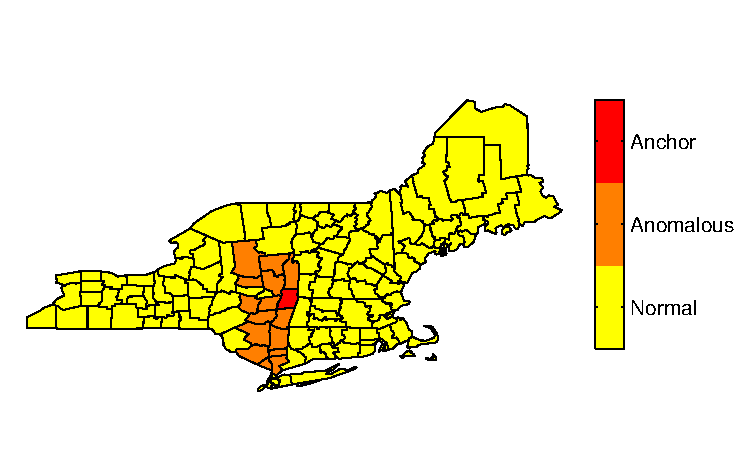
\includegraphics[width=\textwidth]{gt.eps}
        \caption{Ground truth anomalous cluster and anchor node.}
    \label{fig:county}
    \end{subfigure}%
    ~ 
    \begin{subfigure}[t]{0.3\textwidth}
        \centering
        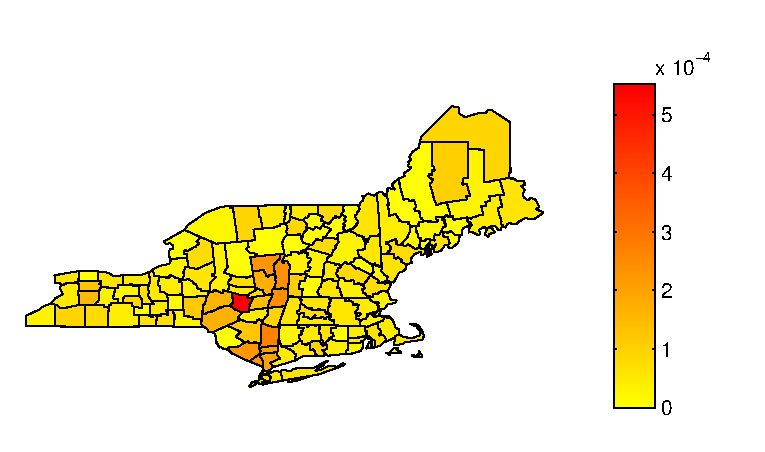
\includegraphics[width=\textwidth]{disease_rates.eps}
        \caption{Sample realization of disease rates for the anomalous case.}
    \label{fig:county_sample}
    \end{subfigure}
    \caption{Disease outbreak detection in northeastern United States counties.}
\end{figure*}

In this section we present experiments on a disease outbreak dataset on a real world geographical network. We compare the statistical detection performance of our mirror descent (MD) algorithm with subgraph detection methods from related work.

The geographical map and corresponding network that we consider are illustrated in Figures \ref{fig:county} and \ref{fig:county_graph} respectively, with 129 nodes representing counties in the northeastern United States and average degree 4.7. The ground truth cluster of 16 nodes for the anomalous case and the chosen anchor node are also illustrated. Note that this dataset has also been considered in \cite{aistats14} and \cite{nips14}, although the network connectivity is slightly different and \cite{aistats14} considers a different ground truth cluster and does not consider detection performance.

Following \cite{disease} and \cite{aistats14,nips14}, we consider an elevated mean Poisson formulation for modeling the diseased population, where the number of disease cases $y_i$ for a county $i$ is given by $y_i \sim \mathrm{Poisson}(N_i \lambda_0)$ where $N_i$ is the population of the county, whereas for anomalous counties we have $y_i \sim \mathrm{Poisson}(N_i \lambda_1)$. We consider $\lambda_0 = 5 \times 10^{-5}$ for the base disease rate and different $\frac{\lambda_1}{\lambda_0}$ ratios $\{1.1, 1.3, 1.5\}$ corresponding to different SNR values. As our test statistic we consider the disease rate per person $x_i = \frac{y_i}{N_i}$. One sample realization for the anomaly case with high SNR $\frac{\lambda_1}{\lambda_0} = 4$ is illustrated in Figure \ref{fig:county_sample}.

To compare the performance with MD as proposed in Algorithm \ref{alg:primaldual}, we consider several other methods in the related literature, including the LMI-test (LMIT) method of \cite{nips14}, simulated annealing (SA) of \cite{duczmal} and the nearest-ball test (NB), which is a parametric method that scans over nearest-neighbor balls for different nodes. For the MD method we consider the optimization value $x x^\top \cdot M$ as the scan statistic, with $T = 100$ iterations, $\eta = 5$ and different $\gamma$ values to quantify the size and conductance of the anomalous graph 

For LMIT we use the same anchor node as MD, anomaly size $|S| = 16$ corresponding to the ground truth and consider scan statistic $x^\top \diag(M)$. We search over a range of values for parameter $\gamma$. For SA and NB we consider the test statistic $\frac{\sum_{i \in S} x_i}{\sqrt{|S|}}$. We initialize SA with the result from NB and run for 40 restarts. 

To quantify detection performance, we threshold the scan statistics given by the algorithms with various threshold values and compute missed detection and false positive rates over a number of samples (50 for MD and LMIT, 25 for SA and NB) generated from both $H_0$ and $H_1$. We then compute the area under the curve (AUC) generated by the pairs of missed detection and false positive rates corresponding to threshold values.

\begin{figure}[ht]
  \centering
  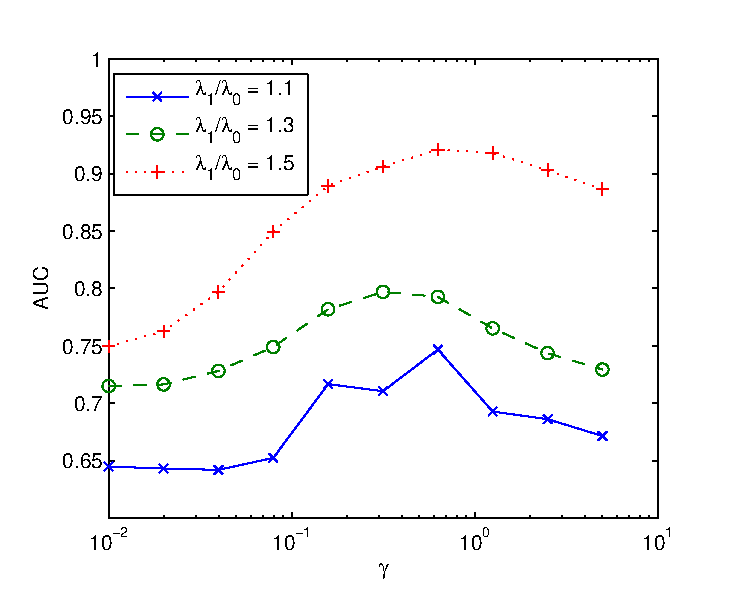
\includegraphics[width=0.4\textwidth]{gammas_auc_curve.eps}
  \caption{Performance of MD algorithm for different $\gamma$ values.}
  \label{fig:gammas}
\end{figure}

\paragraph{Sensitivity of MD to the choice of $\gamma$:} We first investigate the sensitivity of detection performance of MD to $\gamma$, which serves the purpose of parameterizing the internal conductance of candidate subgraphs. We note that unlike \cite{aistats14,nips14}, we do not explicitly specify or search over different cluster sizes, but size information is also implicitly incorporated in $\gamma$. We run MD on the range of values $0.01$ to $5$ in 10 logarithmic intervals. We illustrate the obtained AUC values for different SNR's in Figure \ref{fig:gammas}. 

We observe that while optimal $\gamma$ values differ slightly with different SNR levels, the $0.3$--$0.7$ value range is mostly optimal in all cases. This is in accordance with our expectations, since the size and conductance of the ground truth anomalies do not change across SNR levels.

\paragraph{Comparison to related methods:} We also compare AUC performance of MD to aforementioned methods and tabulate the results in Table \ref{table:auc}. For MD we use a $\gamma$ value of $0.7$ and for LMIT we use a $\gamma$ value of $0.3$ which we observed to perform best empirically. We see that MD performs relatively similar to LMIT, with better performance at some SNR levels. This is expected since the LMI connectivity constraints in both methods are very similar, even though the relaxation to the space of matrices $M$ differ. On the other hand SA and NB perform worse, with SA not significantly improving upon the results of NB. It is also notable that the performance of these three methods seem low when compared to their performance in \cite{nips14} which considered a very similar experimental setup. However this can be partially explained by the different scan statistics used: Aforementioned work utilized the Poisson likelihood test whereas we used the simpler linear form we specified above to be better in line with the scan statistic of MD. It is also possible that the performance of SA can be improved with a larger number of restarts.

\begin{table}[ht]
\centering
\begin{tabular}{| c || c | c | c || c |}
\hline
\multirow{2}{*}{AUC} & \multicolumn{3}{c ||}{$\lambda_1 / \lambda_0$} & \multirow{2}{*}{Runtime} \\
\cline{2-4}
 & 1.1 & 1.3 & 1.5 & \\
 \hline MD & 0.74 & 0.79 & 0.92 & 0.8s \\
 \hline LMIT & 0.65 & 0.81 & 0.86 & 3s \\
 \hline SA & 0.57 & 0.67 & 0.72 & $\sim$3m\\
 \hline NB & 0.57 & 0.67 & 0.68 & 5s\\
 \hline
\end{tabular}
\caption{AUC performance of various algorithms with different SNR values.}
\label{table:auc}
\end{table}

\paragraph{Run-time comparison:} We also provide the average runtime for the recovery methods for a single set of measurements in Table \ref{table:auc}, where the experiments were run on MATLAB on a computer with an Intel i5 4590 processor. We expect that the MD method scale better with larger problems than LMIT that uses cvx/sedumi, which is an off-the-shelf solver for convex problems. We also have not implemented any dimensionality reduction schemes for solving the MD iterations more efficiently as we remarked in Section \ref{sec:MD}.


\section{Conclusion}

We investigated the problem of connected subgraph detection on graph-structured data and proposed an efficient and compact convex relaxation that provably characterizes connectivity and conductance. We then developed a novel iterative optimization method that is provably nearly-linear time in the number of nodes in the graph. We demonstrated its statistical performance on experiments with real world networks, outperforming state-of-the-art methods on the problem while being computationally efficient and scalable.


\vfill
\pagebreak

\appendix
\appendixpage

\section{Proof of Theorem \ref{thm:sufficiency} and an alternative formulation using effective resistance}

In this section we offer an alternative approach to obtain the inequality constraint \eqref{eq:constraint} through electrical networks and the concept of effective resistance. Using this formulation, we then prove Theorem \ref{thm:sufficiency} that shows that the inequality constraint enforces connected through a simple rounding of $M$.

We shortly introduce the concept of effective resistance in the electrical network interpretation of graphs. In contrast to $s$-$t$ flow that interprets edge weights on a graph as flow capacities, electrical flow considers edge weights $w_{ij}$ as the conductance (inverse resistance) $\frac{1}{r_{ij}}$ between two nodes $i,j$.

Define the pseudoinverse of a Laplacian $L^+ = \sum_{i=2}^n \frac{1}{\lambda_i} v_i v_i^\top$ where $L = \sum_{i=2}^n \lambda_i v_i v_i^\top$ is its eigendecomposition, and we note that the minimum eigenvalue $\lambda_1$ corresponding to all $1$ eigenvector is zero. Also note that $L_{G[M]}$ denotes the Laplacian of the subgraph with adjacency matrix $A \odot M$ ($\odot$ is the elementwise/Hadamard matrix product)\footnote{Corresponding to the original graph with edge weights scaled by $M_{ij}$.} and let $L^+_{G[M]}$ denote its pseudoinverse.

Defining a vector of directional current flows into/out of nodes with $f$ (e.g.\ where positive elements are currents into the node and vice versa), the relationship between the vector of voltages $v$ and $f$ in an electrical circuit graph with resistances $r_{ij}$ are given by the relation $v = L^+ f$. This fact follows from Kirchoff's current and voltage laws \cite{Lxb}.
The effective resistance $R_{ab}$ between any two nodes $a, b$ is then defined by the voltage difference $v_a - v_b = v^\top (e_a - e_b)$ when unit current is flowing between two nodes such that $f = e_a - e_b$ (or equivalently, inverse of the current flow with unit voltage difference between $a$ and $b$). We then have the identity $R_{ab} = (e_a - e_b)^\top v = (e_a - e_b)^\top L^+ (e_a - e_b)$.

Given a root/anchor node $r \in V$ that is assumed to be contained in the subgraph $S$, consider the case where a current flow of $d_i M_{ii}$ is present between $r$ and $i \in V$ on the induced graph with Laplacian $L_{G[M]}$. Letting $m_i = d_i M_{ii} (e_r - e_i)$, the voltage vector $v^i$ corresponding to these inputs is given by $v^i = L_{G[M]}^+ m_i$. We then obtain the resistance between nodes $r$ and $i$ for input current $d_i M_{ii}$ with the identity $v^i_r - v^i_i = (e_r - e_i) L_{G[M]}^+ m_i = \frac{1}{d_i M_{ii}} m_i^\top L_{G[M]}^+ m_i$, which we intend to be finite for $i \in S$ (and thus $M_{ii} > 0$) if $G_S$ is connected. For a conductance threshold $\tau$, we would thus like to impose the constraint
\begin{equation}
  m_i^\top L_{G[M]}^+ m_i \leq \frac{d_i M_{ii}}{\tau},
  \label{eq:pair_cond}
\end{equation}
for all $i \in V$, where the scaling with $M_{ii}$ serves to restrict the constraint to only the nodes $i \in S$. We also remark that the constraint \eqref{eq:pair_cond} is independent of uniform multiplicative scaling of $M$, thus constraining $M$ to unit trace does not affect the choice of $\tau$.

We next unify the $n$ different resistance constraints to a single PSD constraint.
Define the $2n \times 2n$ matrix $\mathcal{A}_M$ as
\[ \mathcal{A}_M = \begin{pmatrix} L_{G[M]} & L_{\Star^{(r)}[M]} \\ L_{\Star^{(r)}[M]} & \frac{1}{\tau} L_{\Star^{(r)}[M]} \end{pmatrix}, \]
for which we define our connectivity constraint to be $\mathcal{A}_M \succeq 0$. For $i \neq r$ consider the submatrix $\mathcal{A}_i$ formed by the top-left $n \times n$ submatrix (i.e.\ $L_{G[M]}$) and the $(n+i)$-th row and column, which results in
\[ \mathcal{A}_i = \begin{pmatrix} L_{G[M]} & m_i^\top \\ m_i & \frac{d_i M_{ii}}{\tau} \end{pmatrix}. \]
Since $\mathcal{A}_M \succeq 0$ it implies that any such submatrix satisfies $\mathcal{A}_i \succeq 0$ and through the Schur complement condition that is equivalent to condition \eqref{eq:pair_cond}. We have thus shown that the condition $\mathcal{A}_M \succeq 0$ encapsulates the pairwise effective resistance constraints of the form \eqref{eq:pair_cond}. We note that we obtain a similar condition for the root node, where with currents $m_r \triangleq \sum_{j \neq r} m_j$ applied to the nodes and a convex combination of voltage differences, $m_r^\top L_{G[M]}^+ m_r$ is being compared to $\frac{\sum_{j \neq r} M_{jj}}{\tau}$.

Finally, we can again utilize the Schur complement condition for positive semidefiniteness and simplify the PSD condition $\mathcal{A}_M \succeq 0$ on the $2n \times 2n$ matrix to a PSD condition on an $n \times n$ matrix, which directly leads to inequality \eqref{eq:constraint} when we replace $\tau$ with $\frac{\gamma^2}{2}$.

Now we prove Theorem \ref{thm:sufficiency} using the above reformulation of \eqref{eq:constraint}. Assume there exists $i \in \hat{S}$ such that there exists no path between $r$ and $i$, i.e., the subgraph $G_{\hat{S}}$ is disconnected. Since $Q_\gamma(M) \succeq 0$, it follows that $\mathcal{A}_M \succeq 0$ and thus $\mathcal{A}_i \succeq 0$ for $\tau = \frac{\gamma^2}{2}$. Through the Schur complement lemma and \eqref{eq:pair_cond} we have that $v_r^i - v_i^i \leq \frac{1}{\tau}$, i.e., that the voltage difference between nodes $r$ and $i$ is finite when a current flow of $d_i M_{ii}$ is applied that is non-zero (since $M_{ii} > 0$). This voltage difference is computed for the graph $G$ with edge weights given by $M_{ij}$. It is easy to see that if this voltage difference is finite, the voltage difference in the original graph $G$ is also finite since $M_{ij}$ are bounded. However a contradiction arises because there exists no path between $i$ and $r$ in $G$ and thus the effective resistance $R_{ri} = (e_r - e_i)^\top L^+ (e_r - e_i)$ is infinite.


\section{Proof of Theorem \ref{thm:line_bound}}

Consider the candidate primal solution $M = \frac{1}{K} 1_S 1_S^\top$ under the hypothesis $H_1$ where $|S| = K$. For an $n$-node line graph it is easy to see that this solution is primal feasible for $\gamma \leq \frac{2}{K^2}$. Then for the Poisson model we have a feasible primal value $E[ x x^\top \cdot M] = \frac{1}{K} E[(\sum_{i \in S} x_i)^2 ] = \mu \lambda + \mu^2 \lambda^2 K$.

We next find a feasible dual solution and compute its value under hypothesis $H_0$. We first consider the anchored problem with anchor node $r = 1$. For simplicity we consider $D = I$ when defining the constraint $Q_\gamma(M)$; however this is not relevant to the asymptotic bound since nodes of the graph have bounded constant degree. 
Letting $\alpha$ be the Lagrange multiplier for $I \cdot M = 1$ and $Y$ be the one for $Q_\gamma(M) \succeq 0$, we can write the dual of the optimization problem \eqref{eq:primal_final} without the $M \geq 0$ constraint:
\[ \max_{M \succeq 0} \min_{\alpha, Y \succeq 0} \alpha (1 - I \cdot M) + Y \cdot Q_\gamma(M),\]
which can be rewritten as
\[ \max_{M \succeq 0} \min_{\alpha, Y \succeq 0} \alpha + \left( x x^\top - \alpha I + \sum_{(i,j) \in E} (Y \cdot L_{ij}) e_{ij} - \gamma \sum_{j \neq r} (Y \cdot L_{rj}) e_{jj} \right) \cdot M.\]
Then the dual problem to the original optimization can be written as
\begin{equation}\label{eq:proof_dual}
  \min_{\alpha, Y \succeq 0} \alpha \quad \mathrm{ s.t. } \quad x x^\top + \sum_{(i,j) \in E} (Y \cdot L_{ij}) e_{ij} - \gamma \sum_{j \neq r} (Y \cdot L_{rj}) e_{jj} \preceq \alpha I.
\end{equation}
Furthermore considering dual variables of the form $Y = v v^\top$, a more constrained version of the above problem is given by
\[ \min_{\alpha, v} \, \alpha \quad \mathrm{ s.t. } \quad x x^\top + \sum_{(i,j) \in E} (v_i - v_j)^2 e_{ij} - \gamma \sum_{j = 1}^n (v_r - v_j)^2 e_{jj} \preceq \alpha I. \]

Assume $G$ is a line graph on $n$ nodes, $r = 1$ and let $v_i = \Delta (i-1)$ be the linearly increasing ``voltages'' on the nodes. Then, for the dual constraint we have
\[ x x^\top + \Delta^2 A_{\mathrm{line}} - \gamma \Delta^2 \diag([0,1,\ldots,n-1]) \preceq \alpha I,\]
where $A_{\mathrm{line}}$ is the adjacency matrix of the line graph $G$. Note that $A_{\mathrm{line}} = A_{\mathrm{line}} - D_{\mathrm{line}} + D_{\mathrm{line}} = D_{\mathrm{line}} - L_{\mathrm{line}} \preceq D_{\mathrm{line}} = d I$ where $d = 2$ is the upper bound on the node degrees. Then a sufficient condition for the above constraint to be satisfied is
\[ x x^\top - \gamma \Delta^2 \diag([0,1,\ldots,n-1]) \preceq (\alpha - d \Delta^2) I.\]

We are now interested in the maximum eigenvalue $\lambda_{\max}$ of the left-hand side of the constraint, as that will give a lower bound $\alpha \geq d \Delta^2 + \lambda_{\max}$ which immediately gives a feasible $\alpha$ value along with a feasible $Y = v v^\top$ with the defined voltages. This in turn provides an upper bound on the optimal dual value of \eqref{eq:proof_dual} and thus on the optimal value of the primal \eqref{eq:primal_final}.

We note that the left-hand side is a matrix that is a rank-one matrix $x x^\top$ plus a diagonal matrix $-\gamma \Delta^2 \diag([0,1,\ldots,n-1])$. The eigenvalues of such a matrix must satisfy the following equality \cite{golub}:
\[ f_\Delta(\lambda) \triangleq \sum_{i=0}^{n-1} \frac{x_{i+1}^2}{\lambda + \gamma \Delta^2 i^2} = 1. \]
Note that $f_\Delta(\lambda)$ is a decreasing function of $\lambda$ for positive values and we can assume that $\lambda_{\max} > 0$ (the converse leads to a trivial bound with $\alpha = 0$ feasible). This implies that if there exists $\lambda_0 > 0$ such that $f_\Delta(\lambda_0) \leq 1$, then $\lambda_{\max} \leq \lambda_0$. %By choosing $\Delta$ appropriately, we will show that there exists such a $\lambda_0$.

Note that we can upper bound $f_\Delta(\lambda)$ with
\begin{align*}
  f_\Delta(\lambda) & \leq \frac{x_{\max}^2}{\gamma \Delta^2} \sum_{i=0}^{n-1} \frac{1}{\lambda_\Delta + i^2} \leq \frac{x_{\max}^2}{\gamma \Delta^2} \int_{0}^{n} \frac{1}{\lambda_\Delta + z^2} \dx z \\
  & = \frac{x_{\max}^2}{\gamma \Delta^2 \sqrt{\lambda_\Delta}} \arctan\frac{n}{\sqrt{\lambda_\Delta}} = \frac{x_{\max}^2}{\Delta \sqrt{\gamma \lambda}} \arctan\frac{n \Delta \sqrt{\gamma}}{\sqrt{\lambda}}, \\
  & \leq \frac{\pi x_{\max}^2}{2 \Delta \sqrt{\gamma \lambda}},
\end{align*}
where we defined $\lambda_\Delta \triangleq \frac{\lambda}{\Delta^2 \gamma}$ and used the fact that $\arctan (\cdot) \leq \frac{\pi}{2}$. Then it is clear that $f_\Delta(\lambda_0) \leq 1$ for $\lambda_0 = \frac{\pi^2 x_{\max}^4}{4 \Delta^2 \gamma}$. 

Finally, we have that
\[ \alpha = d \Delta^2 + \frac{\pi^2 x_{\max}^4}{4 \Delta^2 \gamma} = \pi x_{\max}^2 \sqrt{\frac{d}{\gamma}}, \]
as a feasible solution to the dual by choosing $\Delta^2 = \frac{\pi x_{\max}^2}{2 \sqrt{d \gamma}}$.

%Note that $M = \frac{1}{K} 1_S 1_S^\top$ for $|S| = K$ is a feasible solution for the primal problem when $\gamma = \frac{2}{K^2}$ since $L(A_S) - \gamma L_{star} \succeq 0$ (see Lemma 8 in \cite{nips_supp}). The primal optimal value is upper bounded by the dual feasible value $\alpha = \pi x_{\max}^2 K$ for the chosen $\gamma$. We thus need to show that primal value $x x^\top \cdot M = \frac{\left( \sum_{i \in S} x_i \right)^2}{K}$ with above $M$ under the existence of such a set $S$ is asymptotically greater than $\pi x_{\max}^2 K$ under the null hypothesis to show that detection works.

%\subsection*{Improved bound}

We next improve upon the previous bound on $\alpha$.
Assume $K \log^2 n < n$, $K \geq \log n$, let $K_n \triangleq K \log^2 n$ for brevity and $\bar{x}$ such that $\max_{i=1,\ldots,n} x_i^2 \leq \bar{x}^2 \log^2 n$ w.h.p. Also let $\Delta^2 = \bar{x}^2 K \log^2 K$ and $\gamma = \frac{2}{K^2}$. Note that we can write
\[ f_\Delta(\lambda) = \sum_{i=0}^{K_n-1} \frac{x_{i+1}^2}{\lambda + \gamma \Delta^2 i^2} + \sum_{i=K_n}^{n-1} \frac{x_{i+1}^2}{\lambda + \gamma \Delta^2 i^2}. \] 

We first analyze the second term, for which we have
\begin{align*}
  \sum_{i=K_n}^{n-1} \frac{x_{i+1}^2}{\lambda + \gamma \Delta^2 i^2} & \leq \frac{\bar{x}^2 \log^2 (n-K_n)}{\gamma \Delta^2} \int_{K_n}^n \frac{1}{\lambda_\Delta + x^2} \dx x \\
  & = \frac{\bar{x}^2 \log^2 (n-K_n)}{\gamma \Delta^2 \sqrt{\lambda_\Delta}} \left( \arctan \left(\frac{n}{\sqrt{\lambda_\Delta}}\right) - \arctan \left(\frac{K_n}{\sqrt{\lambda_\Delta}}\right) \right) \\
  & = \frac{\bar{x}^2 \log^2 (n-K_n)}{\gamma \Delta^2} \left( \frac{1}{K_n} - \frac{1}{n} - O\left(\frac{1}{K_n^3}\right) \right),
\end{align*}
where the last equality assumes $\frac{K_n}{\sqrt{\lambda_\Delta}} \to \infty$, which we will argue with our choice of $\lambda$. Replacing the quantities with chosen scalings, we then have
\begin{align*}
  \sum_{i=K_n}^{n-1} \frac{x_{i+1}^2}{\lambda + \gamma \Delta^2 i^2} & \leq \frac{K \log^2 (n-K_n)}{2 \log^2 K} \left( \frac{1}{K_n} - \frac{1}{n} - O\left(\frac{1}{K_n^3}\right) \right) \\
  & = O\left( \frac{K \log^2 (n-K_n)}{K_n \log^2 K} \right) = O\left(\frac{1}{\log^2 K}\right).
\end{align*}

The analysis of the first term follows along the lines of the previous bound, with $n$ replaced by $K_n$, where we have the upper bound
\begin{align*}
  \sum_{i=0}^{K_n-1} \frac{x_{i+1}^2}{\lambda + \gamma \Delta^2 i^2} & \leq \frac{\bar{x}^2 \log^2 K_n}{\gamma \Delta^2} \int_0^{K_n} \frac{1}{\lambda_\Delta + z^2} \dx z \\
  & \leq \frac{\bar{x}^2 \log^2 K_n}{\sqrt{\gamma \Delta^2 \lambda}} \frac{\pi}{2} = \frac{\bar{x} \sqrt{K} \log^2 K_n}{\log K \sqrt{\lambda}} \frac{\pi}{2\sqrt{2}}.
\end{align*}

Letting $\lambda_0 = 4.5 \pi^2 \bar{x}^2 K \log^2 K$, we see that the first term can be upper bounded by $\frac{\log^2 K_n}{9 \sqrt{2} \log^2 K} \leq \frac{1}{\sqrt{2}}$ with the assumption that $K \geq \log n$ thus $\frac{\log (K\log^2 n)}{\log K} \leq 3$. We also observe that $\lambda_\Delta = \frac{\lambda_0}{\gamma \Delta^2} = 2.25 \pi^2 K^2$, thus satisfying the condition $\frac{K_n}{\sqrt{\lambda_\Delta}} \to \infty$ that we used while analyzing the second term. Thus we have that
\[ f_\Delta(\lambda_0) \leq \frac{1}{\sqrt{2}} + O\left( \frac{1}{\log^2 K} \right) < 1,\]
for the above choice of $\lambda_0$, which leads to 
\[ \alpha = d \Delta^2 + \lambda_0 = (d + 4.5 \pi^2) \bar{x}^2 K \log^2 K, \]
as a feasible dual value.

Finally note that under the $H_0$ hypothesis, $\bar{x}^2 \leq \lambda + \lambda^2$ due to the concentration of the Poisson variables. Considering a constant $\lambda$, we then have an upper bound to the dual optimal value under $H_0$, $\alpha = O(K \log^2 K)$. It then follows from standard concentration results that $\mu = \Omega(\log K)$ is sufficient to obtain asymptotic separability between the primal optimal under $H_1$ and primal optimal under $H_0$. It then follows directly from union bounding over different anchor nodes $r = 1,\ldots,n$ that $\mu = \Omega(\log K \sqrt{\log n})$ is sufficient in the anchor-agnostic case.


\clearpage
\Urlmuskip=0mu plus 1mu\relax

\bibliographystyle{icml2017}
\bibliography{subgraph}

\end{document}


